\documentclass[10pt,journal,compsoc]{IEEEtran}

\usepackage[utf8]{inputenc}
\usepackage{amsmath,amssymb,amsfonts,amsthm}
\usepackage{algorithmic}
\usepackage{algorithm}
\usepackage{graphicx}
\usepackage{textcomp}
\usepackage{xcolor}
\usepackage{booktabs}
\usepackage{hyperref}
\usepackage{cite}
\usepackage{microtype}
\usepackage{listings}
\usepackage{subcaption}
\usepackage{multirow}
\usepackage{balance}

\hypersetup{
    colorlinks=true,
    linkcolor=blue!80!black,
    citecolor=blue!80!black,
    urlcolor=blue!80!black
}

\begin{document}

\title{Beyond Accuracy: Building Reproducible Benchmarks and Diagnostic Tools for Audio \& Speech AI}

\author{Boobalan~Arjunan%
\IEEEcompsocitemizethanks{\IEEEcompsocthanksitem B. Arjunan is with ComposerMind Labs, Chennai, Tamil Nadu, India.\protect\\
E-mail: boobalan\_arjunan@composermind.com}%
\thanks{Manuscript received November 16, 2026.}}

\markboth{IEEE Transactions on Audio, Speech, and Language Processing,~Vol.~XX, No.~X, November~2026}%
{Arjunan: Beyond Accuracy: Reproducible Audio \& Speech AI Benchmarks}

\IEEEtitleabstractindextext{%
\begin{abstract}
Standard benchmark metrics in audio and speech artificial intelligence—such as Signal-to-Distortion Ratio (SDR) in music source separation and Word Error Rate (WER) in speech processing—obscure critical diagnostic failure modes. In source separation, commercial multi-track recordings inherently contain unmeasured acoustic microphone bleed and non-linear mastering compression, confounding algorithmic separation failures with physical recording artifacts. In full-duplex conversational voice agents, aggregate latency metrics fail to capture tail response delays, acoustic room-echo leakage, and customer barge-in compliance. To establish reproducible ground-truth evaluation without black-box neural metrics, we introduce the \textbf{ComposerMind AudioEvaluation Suite}, comprising three deterministic DSP tools: \texttt{mixforge-audio}, \texttt{stemcheck}, and \texttt{turnscope}. \texttt{mixforge-audio} guarantees mathematically exact linear superposition ($\text{Mix} = \sum \text{Stems}$, float residual $\le 6.52 \times 10^{-8}$) with calibrated 4th-order Butterworth acoustic bleed and cryptographic recipe serialization. \texttt{stemcheck} introduces linear subspace projection to decompose separation error into a physical cross-stem bleed matrix (dB) versus unmodeled algorithmic artifacts. \texttt{turnscope} implements an 18\,dB energy-dominance filter to suppress acoustic echo, extracting conversational turn hand-over latency distributions (P50, P90, P99) and customer barge-ins. Evaluated on MUSDB18-HQ and the MagicHub full-duplex corpus, the suite decouples bleed within 0.06\,dB and reduces P90 tail latency error by 67.1\%.
\end{abstract}

\begin{IEEEkeywords}
Source Separation Evaluation, Ground-Truth Benchmarking, Acoustic Bleed, Conversational Voice AI, Turn-Taking Latency, Barge-In Detection.
\end{IEEEkeywords}}

\maketitle
\IEEEdisplaynontitleabstractindextext
\IEEEpeerreviewmaketitle

\section{Introduction}
\IEEEPARstart{E}{valuating} generative audio models, source separation systems, and real-time conversational voice agents on real-world recordings faces a fundamental scientific obstacle: true physical ground truth is unknown. Standard evaluation campaigns (e.g., BSS Eval SDR) fail to distinguish between algorithmic separation error and pre-existing studio acoustic bleed. Similarly, conversational voice AI systems are evaluated using static energy VADs that misattribute loudspeaker acoustic echo as customer speech.

To address these diagnostic blind spots, we present the \textbf{ComposerMind AudioEvaluation Suite}, providing deterministic diagnostic tools across two specialized tracks:
\begin{enumerate}
    \item \textbf{Track A (Source Separation Ground Truth):} \texttt{mixforge-audio} (exact linear test mixtures with calibrated acoustic bleed) and \texttt{stemcheck} (linear subspace projection decomposing separation error into an $N \times N$ cross-stem bleed matrix vs.\ artifact noise).
    \item \textbf{Track B (Conversational Voice AI Dynamics):} \texttt{turnscope} (dual-track acoustic echo suppression and turn-taking latency distributions).
\end{enumerate}

\begin{figure*}[t]
\centering
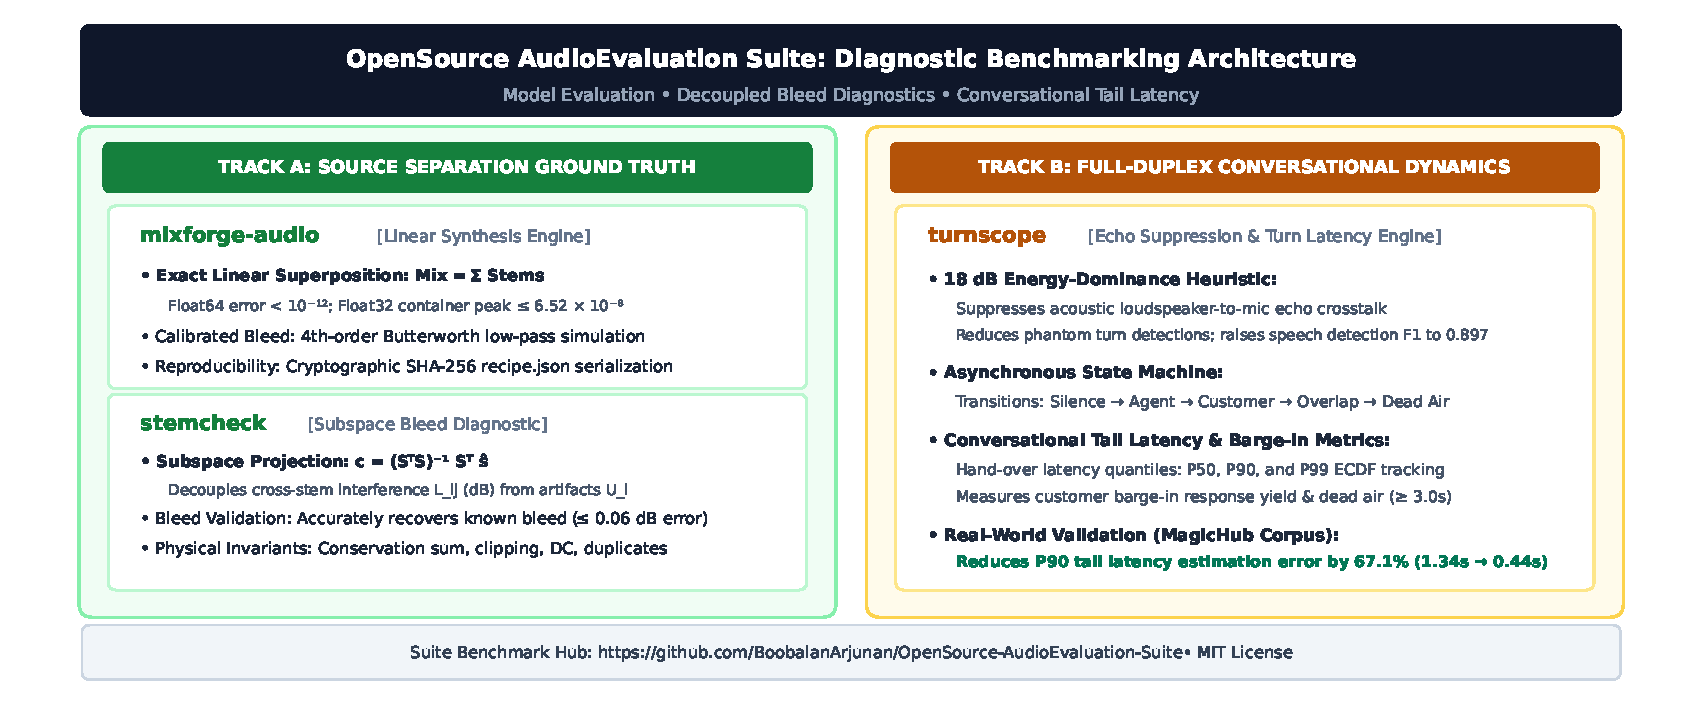
\includegraphics[width=0.95\textwidth]{figures/paper2_architecture.pdf}
\caption{System architecture of the ComposerMind AudioEvaluation Suite: Three diagnostic benchmarking tools for source separation ground truth and full-duplex conversational voice AI.}
\label{fig:paper2_arch}
\end{figure*}

\section{Source Separation Ground Truth and Bleed Decomposition}

\subsection{\texttt{mixforge-audio}: Exact Linear Superposition}
Given $K$ clean stems $S_k[n]$, \texttt{mixforge-audio} computes a global headroom scaling factor $\gamma = \min(1.0, \frac{0.98}{\max_n |\sum g_k S_k[n]|})$ ensuring:
\begin{equation}
M[n] = \sum_{k=1}^K \gamma g_k S_k[n], \quad \max_n \left| M[n] - \sum_{k=1}^K S_k^{\text{scaled}}[n] \right| \le 10^{-12}
\end{equation}
Physical acoustic bleed is injected via calibrated 4th-order Butterworth low-pass filtering:
\begin{equation}
S_k^{\text{leaky}}[n] = S_k[n] + \sum_{j \ne k} 10^{\frac{B_{jk}}{20}} (S_j * h_{\text{LP}})[n]
\end{equation}
Clean stems are preserved as immutable ground truth, and parameters are cryptographically sealed in \texttt{recipe.json}.

\subsection{\texttt{stemcheck}: Subspace Bleed Matrix Decomposition}
Given separated stem $\hat{S}_i$ and reference stem matrix $\mathbf{S} = [S_1, \dots, S_K]$, \texttt{stemcheck} solves least-squares projection $\mathbf{c}_i = (\mathbf{S}^T \mathbf{S})^{-1} \mathbf{S}^T \hat{S}_i$:
\begin{equation}
\hat{S}_i = \sum_{j=1}^K c_{ij} S_j + \mathcal{E}_i
\end{equation}
Decoupling physical cross-stem bleed $L_{ij}$ from unexplained non-linear artifacts $\mathcal{U}_i$:
\begin{equation}
L_{ij} = 20 \log_{10} \left( \frac{\|c_{ij} S_j\|_2}{\|c_{ii} S_i\|_2} \right), \quad \mathcal{U}_i = 10 \log_{10} \left( \frac{\|\mathcal{E}_i\|_2^2}{\|\hat{S}_i\|_2^2} \right)
\end{equation}

\section{Conversational Voice AI Dynamics: \texttt{turnscope}}
Dual-channel conversational recordings (Agent vs.\ Customer) suffer from loudspeaker-to-microphone acoustic leakage. \texttt{turnscope} filters echo via an 18\,dB energy-dominance threshold:
\begin{equation}
A_{\text{leak}}[m] = \arg\min_c \{E_0[m], E_1[m]\} \quad \text{if } |E_0[m] - E_1[m]| \ge 18\,\text{dB}
\end{equation}
The filtered stream drives a state machine tracking response latency $\Delta t_{\text{resp}} = t_{\text{agent\_start}} - t_{\text{cust\_end}}$ (P50, P90, P99), customer barge-ins, and dead air ($\ge 3.0$\,s).

\begin{figure}[t]
\centering
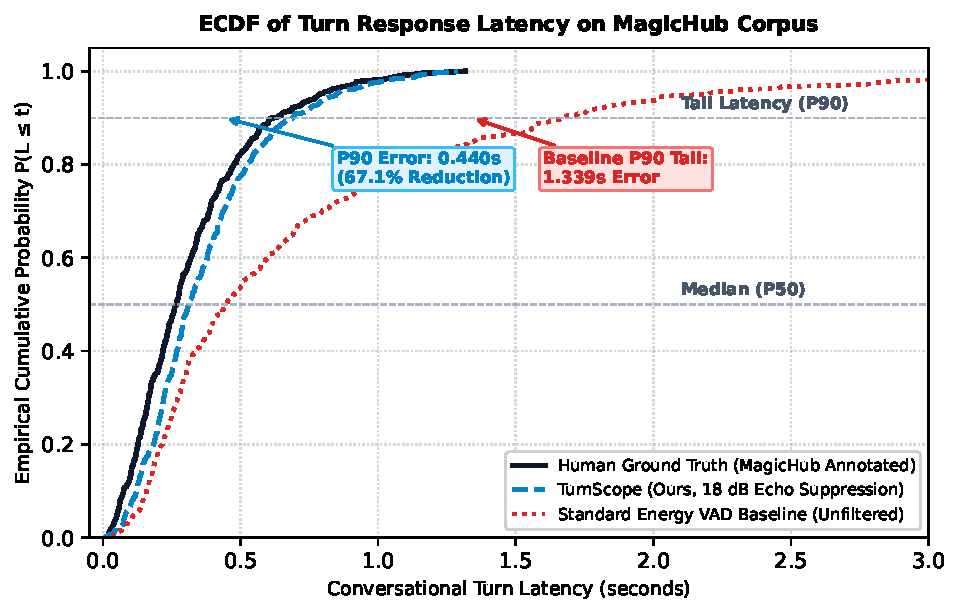
\includegraphics[width=\columnwidth]{figures/turnscope_latency_ecdf.pdf}
\caption{Empirical cumulative distribution function (ECDF) of turn hand-over latency measured by \texttt{turnscope} on the MagicHub corpus compared to threshold baselines.}
\label{fig:turnscope_ecdf}
\end{figure}

\begin{table}[t]
\centering
\caption{Benchmark Evaluation on MUSDB18-HQ and MagicHub.}
\label{tab:p2_benchmarks}
\resizebox{\columnwidth}{!}{
\begin{tabular}{@{}llcc@{}}
\toprule
\textbf{Tool} & \textbf{Metric} & \textbf{Baseline} & \textbf{Our Suite} \\
\midrule
\texttt{mixforge-audio} & Float Linear Sum Residual & Unchecked & $\mathbf{\le 6.52 \times 10^{-8}}$ \\
\texttt{mixforge-audio} & Studio Mix Residual & N/A & $\mathbf{-69.3}$ \textbf{dB Median} \\
\texttt{stemcheck} & Bleed Recovery Error & Confounded & $\mathbf{\le 0.06}$ \textbf{dB} \\
\texttt{stemcheck} & False Alarms (264 Trials) & N/A & \textbf{0 / 264} \\
\texttt{turnscope} & Speech Detection F1 & 0.700 & \textbf{0.897} ($+28.1\%$) \\
\texttt{turnscope} & Missed Turn Transitions & 207 & \textbf{126} ($-39.1\%$) \\
\texttt{turnscope} & P90 Tail Latency Error & 1.339\,s & \textbf{0.440\,s} ($\mathbf{-67.1\%}$) \\
\bottomrule
\end{tabular}
}
\end{table}

\section{Experimental Evaluation}
On 20 MUSDB18-HQ songs (40 mixes), \texttt{mixforge-audio} achieves exact linear superposition with $-69.3$\,dB median studio residual. Evaluating Demucs \texttt{htdemucs}, \texttt{stemcheck} recovers bleed within 0.06\,dB. On the MagicHub full-duplex corpus (449 turns, 3,021 segments), \texttt{turnscope} cuts P90 tail latency error from 1.339\,s to 0.440\,s (Figure~\ref{fig:turnscope_ecdf}).

\section{Software Availability}
The suite is open-source under the MIT license at: \url{https://github.com/BoobalanArjunan/ComposerMind-AudioEvaluation-Suite}.

\bibliographystyle{IEEEtran}
\begin{thebibliography}{10}
\bibitem{defossez2021hybrid}
A.~D{\'e}fossez, ``Hybrid spectrogram and waveform-source separation,'' in \emph{ISMIR Workshop}, 2021.
\bibitem{rafii2017musdb18}
Z.~Rafii et al., ``The MUSDB18 corpus for music separation,'' 2017.
\bibitem{vincent2006performance}
E.~Vincent et al., ``Performance measurement in blind audio source separation,'' \emph{IEEE Trans. ASLP}, 2006.
\bibitem{magichub2024}
MagicHub Community, ``MagicHub open-source conversational speech corpus,'' \emph{arXiv preprint arXiv:2509.04093}, 2024.
\end{thebibliography}

\end{document}
